\headerblock{
  \headerquote{Well-chosen, non-frivolous epigraphs can enhance a thesis.}{Dave Clarke~\cite{AcademiaSE}}
}

\section{Word Clouds}

Here is a word cloud generated from all the text in this thesis.
I used the \githubref{https://github.com/amueller/word\_cloud}{\texttt{wordcloud\_cli} Python tool} on all \verb|.tex| sources and \verb|sed| to crudely filter out LaTeX-related words. In particular, I filtered out comments (anything after \verb|%|), commands (words starting with \verb|/|), and selected arguments
(contents inside \verb|\begin|, \verb|\end|, \verb|\label|, \verb|\ref|, \verb|\cite|, etc.).

\headerblock{
  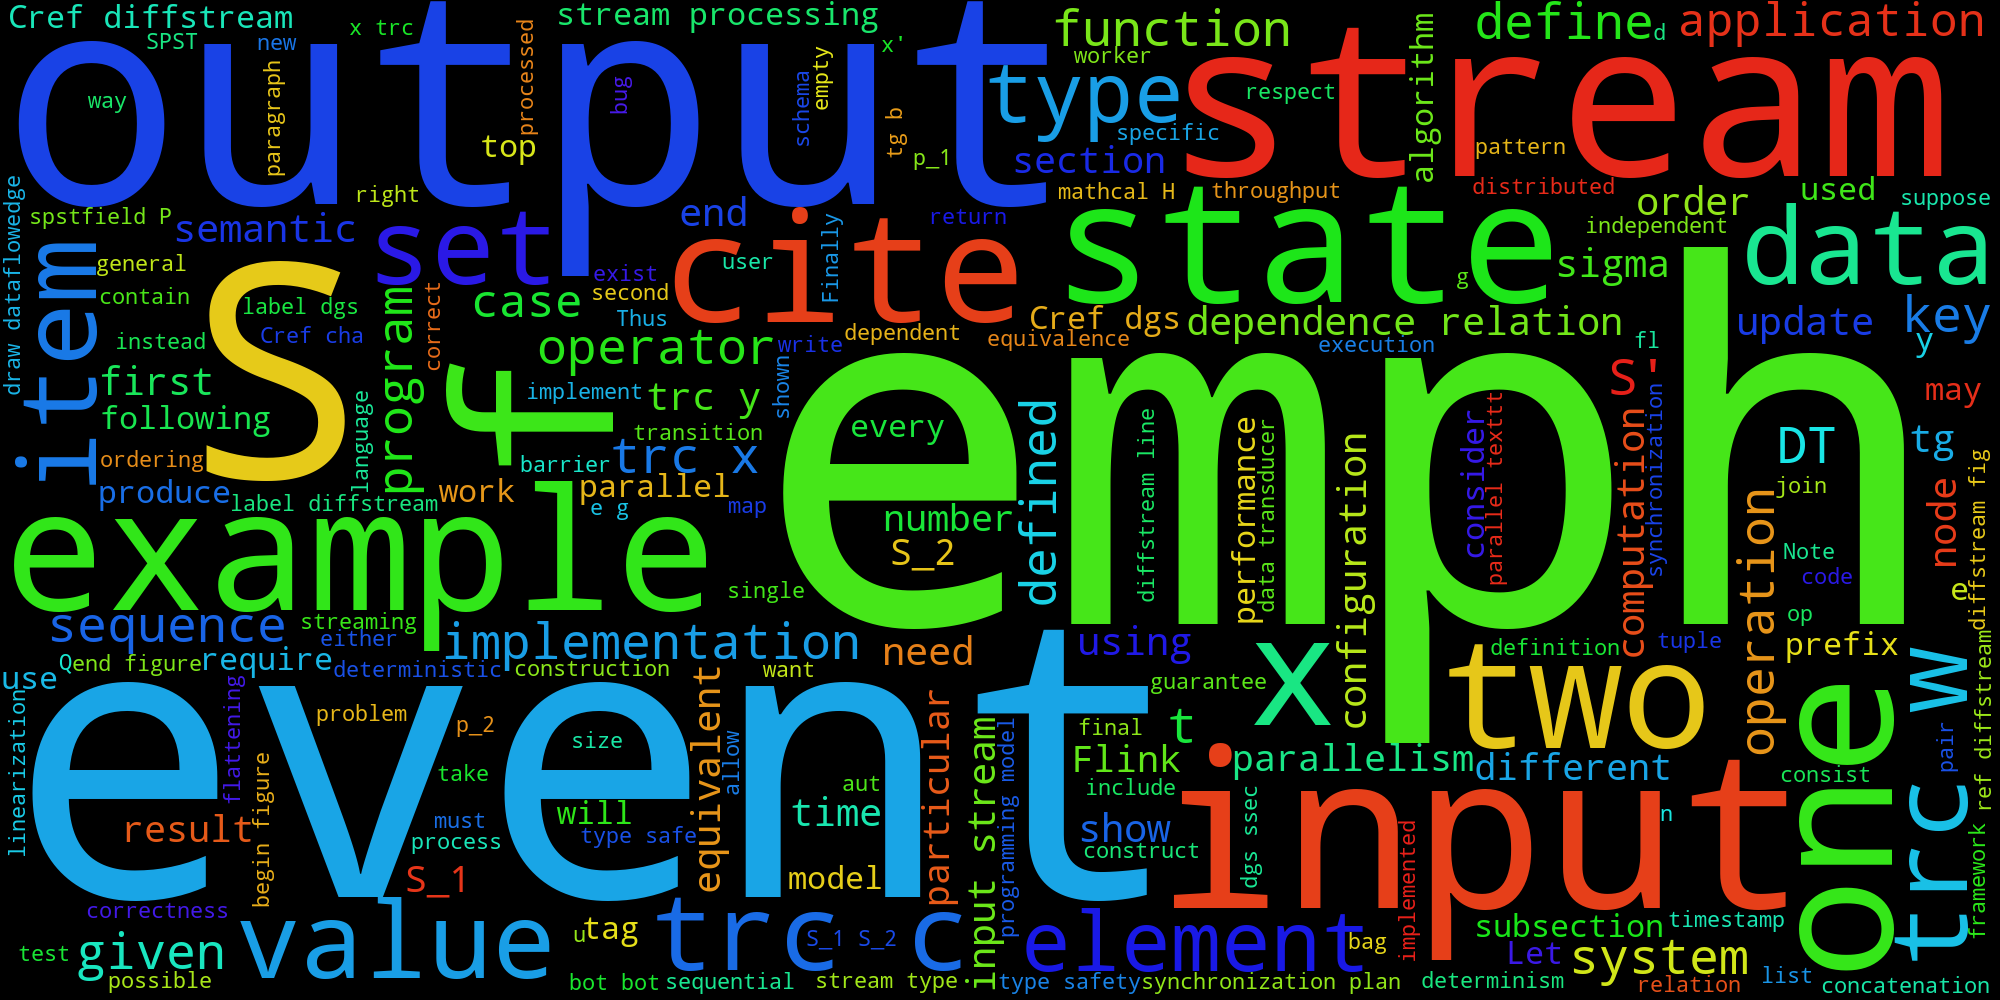
\includegraphics[width=0.6\textwidth]{img/wordcloud.png}
}

And here is a word cloud for the references (bibliography) file.
This only includes text in the \verb|title=| and \verb|author=| fields.

\headerblock{
  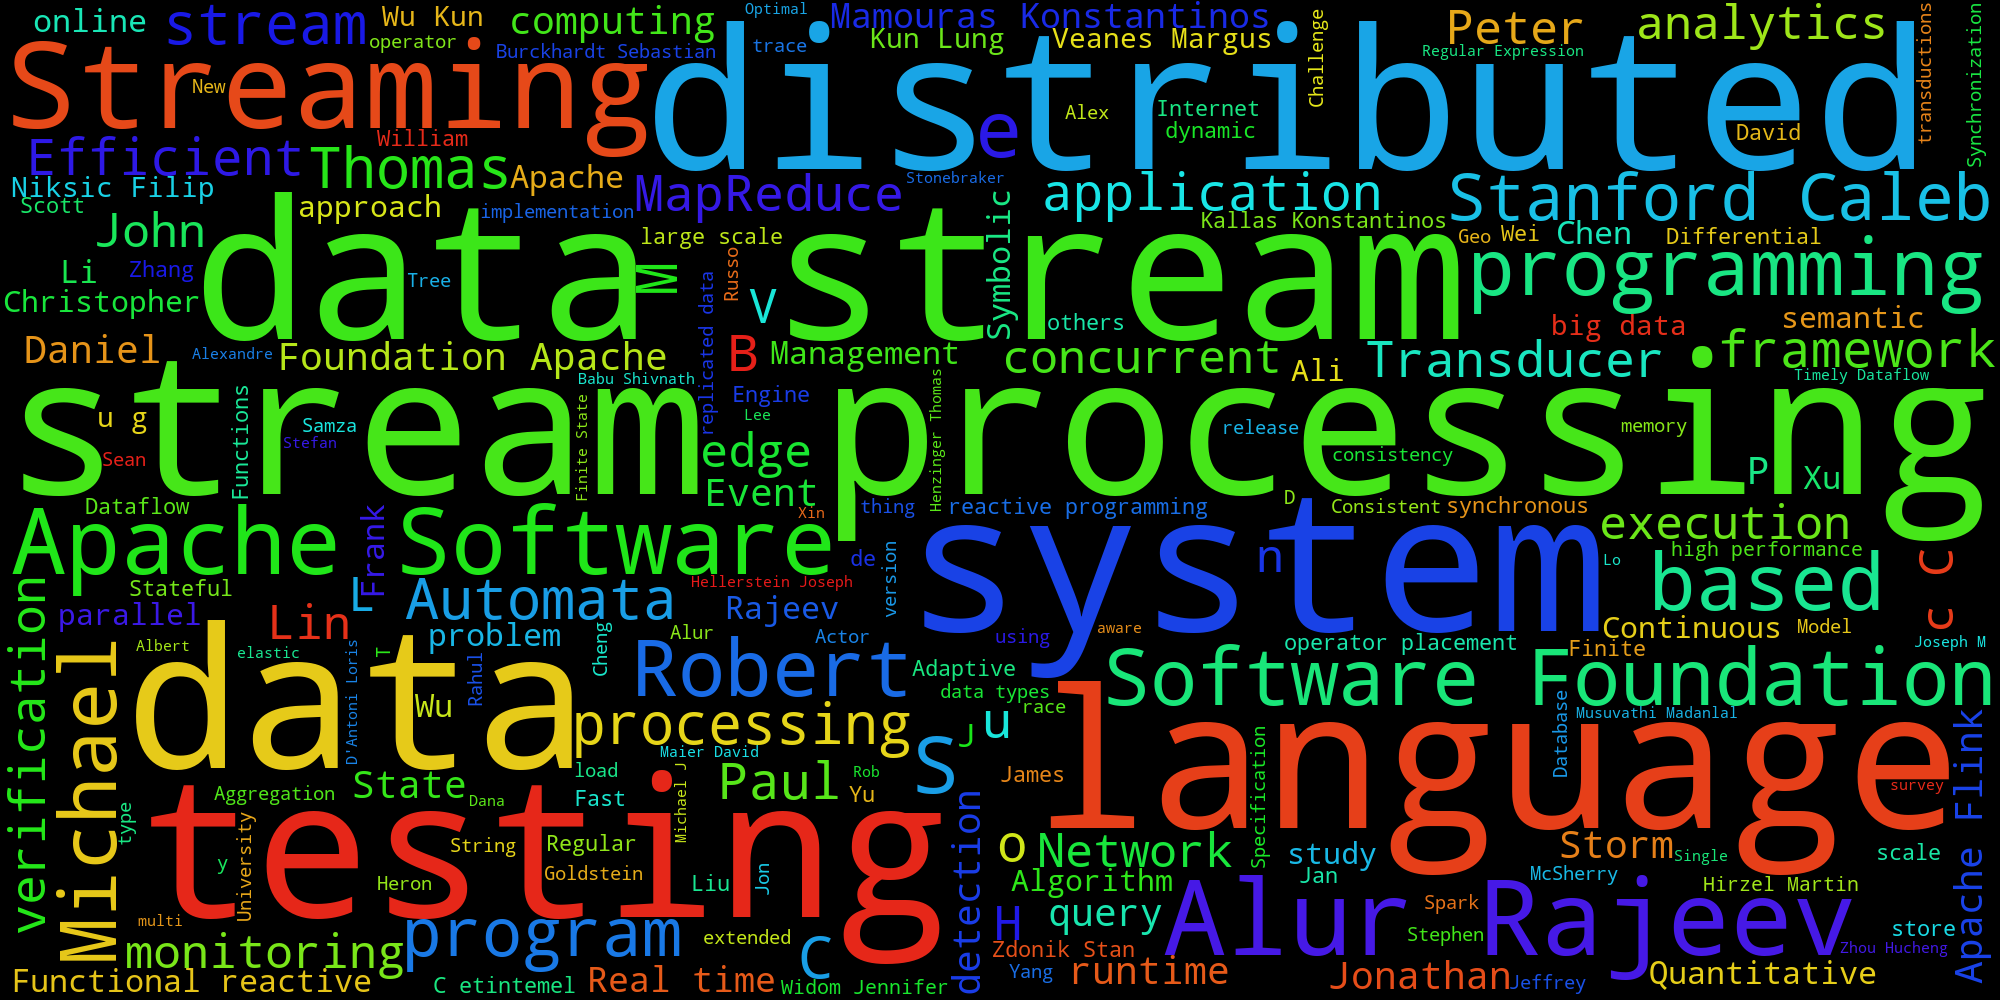
\includegraphics[width=0.6\textwidth]{img/wordcloud_refs.png}
}

\section{Epigraph Outtakes}

\headerblock{
\headerbreak{}
\headerquote{Elegance is not a dispensable luxury but a quality that decides between success and failure.}{Edsger Dijkstra}

\headerbreak{}
\headerquote{Definitions belong to the definers, not the defined.}{Toni Morrison}

\headerbreak{}
\headerquote{A \underline{good} concept is one that is closed
(1) under arbitrary composition
(2) under recursion.}{Gilles Kahn, 1974~\cite{gilles1974semantics}}

\headerbreak{}
\headerquote{The restriction of finiteness appears to give a better approximation to the idea of a physical machine. Of course, such machines cannot do as much as Turing machines, but the advantage of being able to compute an arbitrary general recursive function is questionable, since very few of these functions come up in practical applications.}{Rabin and Scott}

\headerbreak{}
\headerquote{Almost every problem that you come across is befuddled with all kinds of extraneous data of one sort or another; and if you can bring this problem down into the main issues, you can see more clearly what you’re trying to do.}{Claude Shannon}
}

\section{Special Mention}

\bigskip

\begin{center}
  \setlength{\tabcolsep}{10pt}
  \renewcommand{\arraystretch}{3.3}
  \begin{tabular}{cc}
    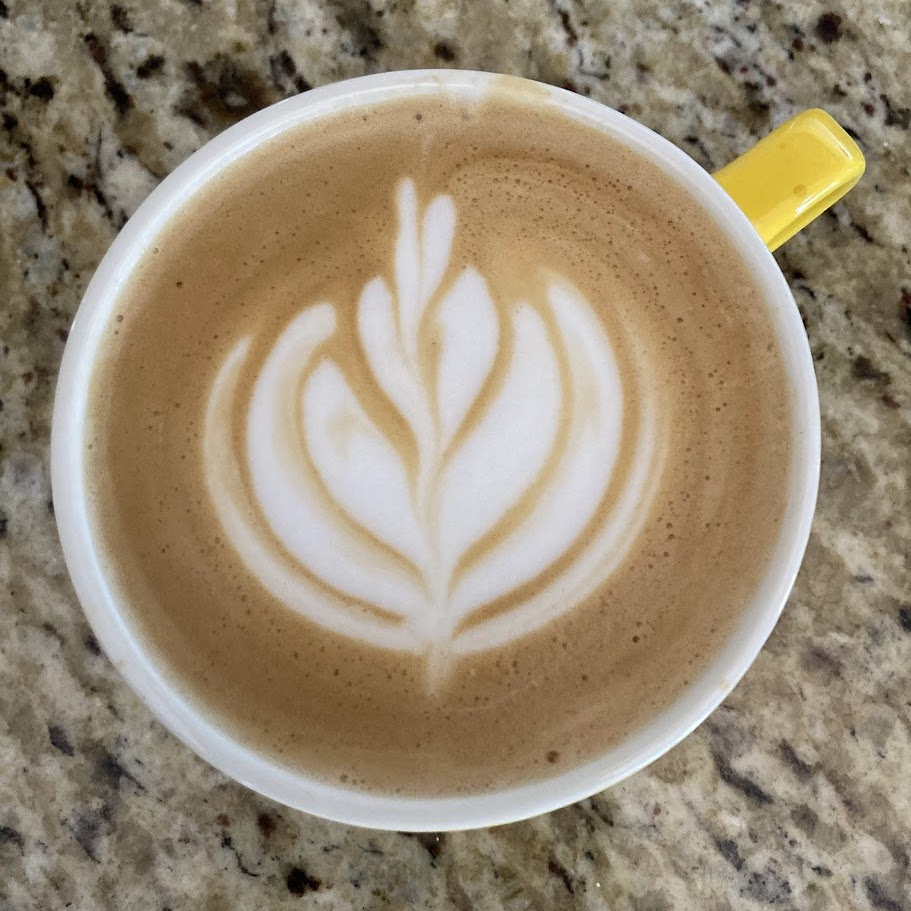
\includegraphics[width=6cm]{img/latte-06-26.jpg} &
    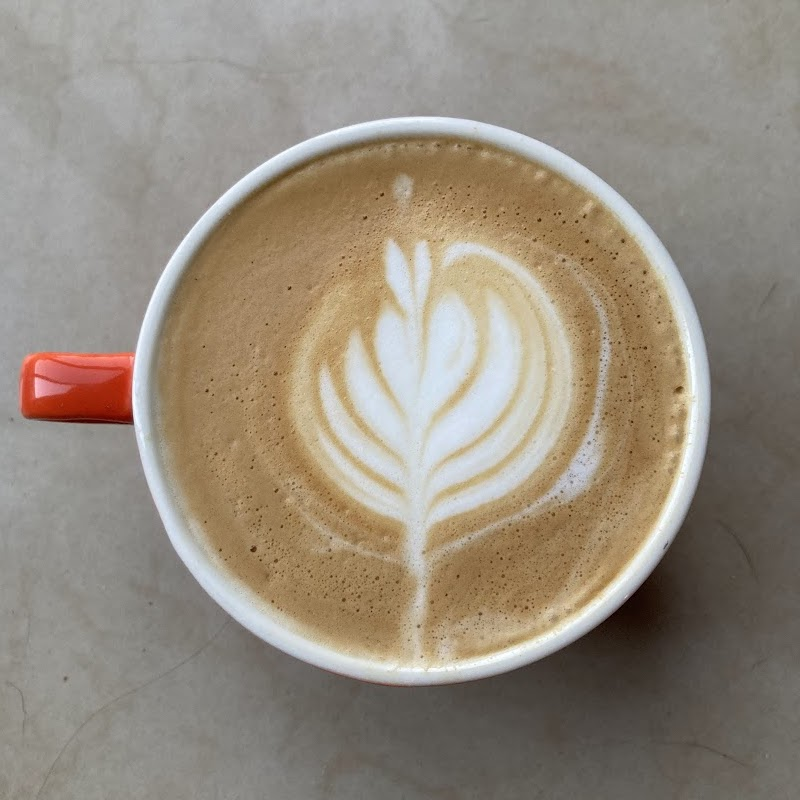
\includegraphics[width=6cm]{img/latte-06-29.jpg} \\
    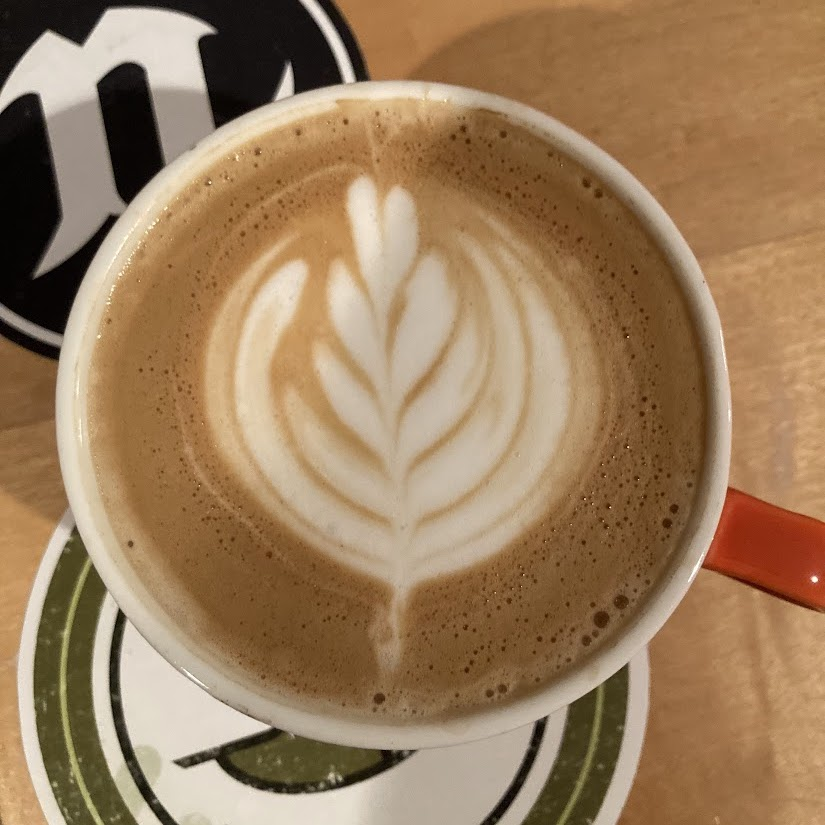
\includegraphics[width=6cm]{img/latte-07-02.jpg} &
    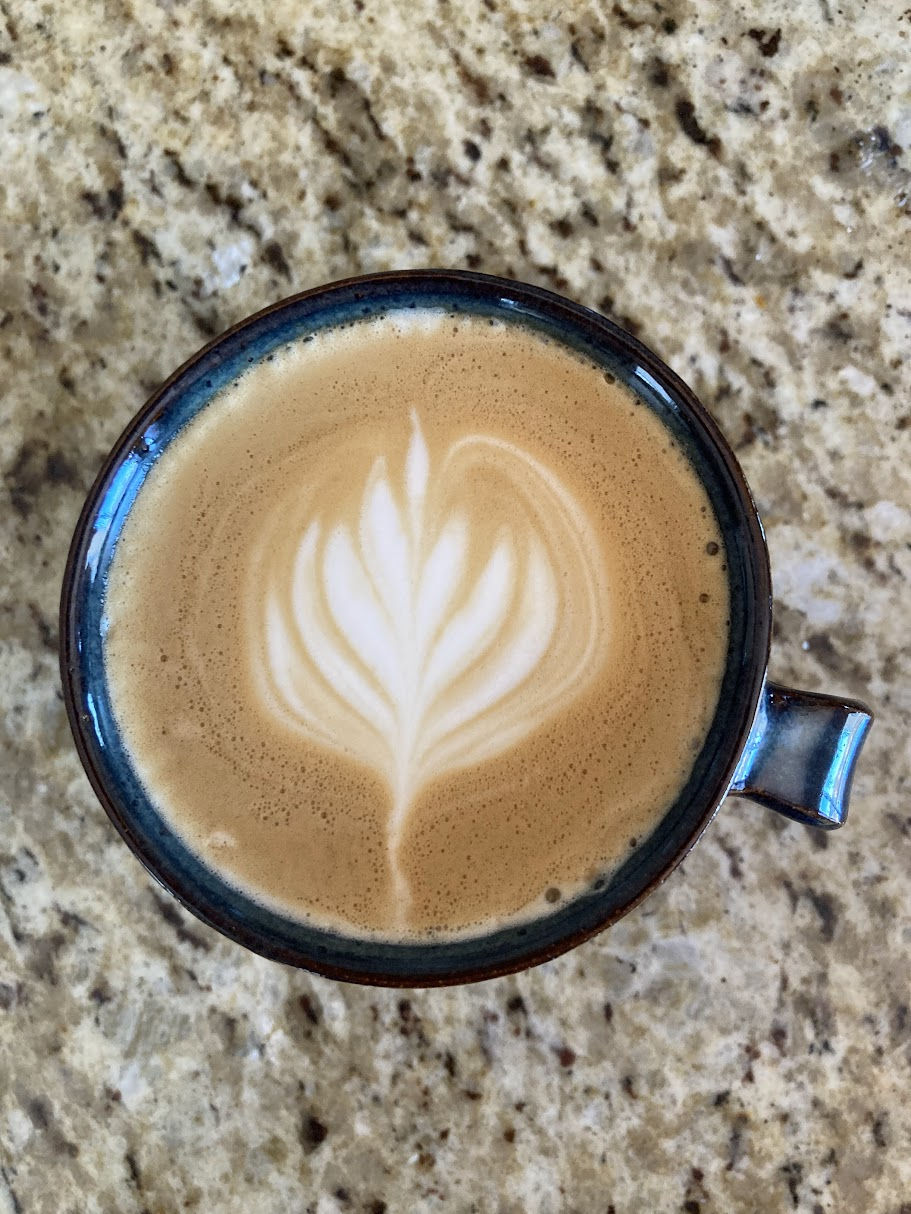
\includegraphics[width=6cm]{img/latte-07-04.jpg} \\
  \end{tabular}
\end{center}
